\section{Medical Subject Heading Over–representation Profiles}
\subsection{Définition}
MeSHOP est une application très complète.Celle-ci permet de centraliser les recherches et d'indexer les publications scientifiques. Celli ci englobe des thématiques allant de la recherche génétique à la chimie en passant par les maladies, ce qui interesse l'auteur.

\subsection{fonctionnement}
Le moteur de cette application repose sur une base de données MEDLINE et le moteur de recherche PubMed.

\iffalse

\includegraphics[width=40mm, height=15mm, scale=0.5]{medline}

\includegraphics[width=25mm,scale=0.5]{pubmed}
\fi

\subsubsection{Annotations}
Chaque article devra être annoté avec un vocabulaire particulier. En effet, c'est cette annotation qui permettra une recherche efficace. Le système MeSH a une liste de vocabulaire (\textit{PMIDs}) qui servira d'index pour le fichier.

\subsection{Editer un article}
Après l'écriture d'un article, il est nécessaire de le publier. Et c'est à ce moment là que va servir le système d'annotation. En effet une lecture par un robot de l'article sera fait et permettra, en fonction du vocabulaire utilisé, de classer l'article dans des catégories et de l'indexer pour des recherches.
\\
\begin{figure}{l}{}
\centering
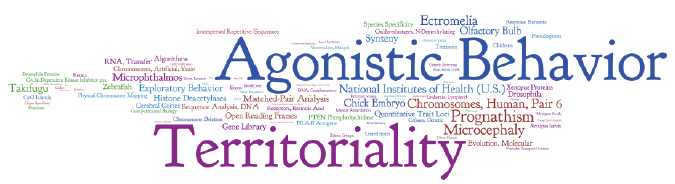
\includegraphics{nuagepoint}
\caption{exemple d'un nuage de mot}
\end{figure}


Chaque mot sera classé en fonction de son nombre d'ocurence dans les \textit{PMIDs}


\subsection{Recherche}
Un point important est la thématique recherchée. En effet, comme vu précédemment, les sujets d'articles englobent un grand nombre de thématique (génétique, maladies, chimie etc...) et donc le contexte peut changer pour des mêmes mots ou combinaisons de mots.